%--------------------------------------------------------------------------------------------------------------------------------%
% Code and text for "A mechanistic model to compare the importance of interrelated population measures: population size, population density and colony size"
% Chapter 4 of thesis "The role of population structure and size in determining bat pathogen richness"
% by Tim CD Lucas
%
%---------------------------------------------------------------------------------------------------------------------------------%












\section{Abstract}

%\tmpsection{One or two sentences providing a basic introduction to the field}
% comprehensible to a scientist in any discipline.
\lettr{A}n increasingly large fraction of emerging diseases come from wild animals and these diseases have a huge impact on human health.
The chance that a new disease will come from any particularly host species increases with the number of pathogen species in that host species.
However, the factors that control pathogen richness in wild populations are still poorly understood.
%\tmpsection{Two to three sentences of more detailed background}
Comparative studies have found evidence that host density, geographic range size and population structure are associated with high pathogen richness. 
Additionally, epidemiological theory suggests that host population structure and host population abundance may influence pathogen richness.
However, these factors are intrinsically linked.
Host density is population size divided by range size while reducing host density directly reduces host population size and reduces contacts between individuals, therefore increasing population structure.
In group living species group size and the total number of groups both contribute to total host population size. 
As these factors are all completely interdependent, it is impossible to identify the causal factors within a comparative frame work.
%\tmpsection{One sentence clearly stating the general problem (the gap)}
% being addressed by this particular study.
%\tmpsection{One sentence summarising the main result}
%  (with the words ``here we show'' or their equivalent).
Here I use metapopulation susceptible-infected-recovered (SIR) models to test whether it is host density \emph{per se} that increases the ability of a newly evolved pathogen to invade and persist in a population as opposed to host group size, population size or range size.
I parameterised these metapopulations to mimic bat populations as bats exhibit a large range in group (colony) size and geographic range size as well as being associated with a number of important zoonotic pathogens.
%\tmpsection{Two or three sentences explaining what the main result reveals in direct comparison to what was thought to be the case previously}
% or how the main result adds to previous knowledge
%\tmpsection{One or two sentences to put the results into a more general context.}
I found that increased population size increased the chance that a new pathogen will invade into a population more than host density.
Furthermore, increased group size increased the probability of pathogen invasion more than the number of groups.
This implies that, in comparative studies, host density may be merely a correlate of group size or population size.
%\tmpsection{Two or three sentences to provide a broader perspective, }
% readily comprehensible to a scientist in any discipline.
This study helps clarify both the inter-relationships between, and relative importance of, a number of host, population-level factors affecting pathogen richness. 
It also highlights the necessity for studying the mechanisms underlying pathogen community construction as comparative approaches do not have the specificity to do so.



%%%%%%%%%%%%%%%%%%%%%%%%%%%%%%%%%%%%%%%%%%%%%%%%%%%%%%%%%%%%%%%%%%%%%%%%%%%%%%%%%%%%%%%%%%%%%%%%%%%%%%%%%%%%%%%%%%%%%%%%%%%%%%%%%%%%%%%%%%%%%%%%%%%%%%%%%%%


\section{Introduction}

%%%%%%%%%%%%%%%%%%%%%%%%%%%%%%%%%%%%%%%%%%%%%%%%%%%%%%%%%%%%%%%%%%%%%%%%%%%%%%%%%%%%%%%%%%%%%%%%%%%%%%%%%%%%%%%%%%%%%%%%%%%%%%%%%%%%%%%%%%%%%%%%%%%%%%%%%%%


%This is quite a good introduction but I think the order is a bit mixed up - you are first talking about mechanistic studies and then comparative studies and then go back into mechanistic studies but this is far from clear and it is a confusing read at the moment

%I would suggest the following structure
%1. Zoonotics important - determinants of pathogen richness important
%2. review the evidence for comparative studies for size and other interrelated variables  first as that is the order you do it in other chapters
%3. But other interrelated variables and problems with definitions
%4. Problems can't be fixed with a comparative approach
%5. review the evidence for mechanistic studies
%6. limitations of the mechanistic approach so far
%7. what you are going to do that is new (ie tease apart these interdependencies) - using case study on bats (and why this is a good group to ask this particular question on)





\tmpsection{General Intro}
%%%%%%%%%%%%%%%%%%%%%%%%%%%%%%
% A basic introduction to the field,
% comprehensible to a scientist in any discipline.

%1. Zoonotics important - determinants of pathogen richness important

Zoonotic diseases are an increasingly important source of human infectious diseases \cite{jones2008global, woolhouse2006host, taylor2001risk}.
The chance that a new zoonotic disease will come from a particular host reservoir depends on a number of factors including the number of pathogen species it carries \cite{wolfe2000deforestation}.
It is well known that population-level factors such as host density, range size and population structure have an important role in controlling pathogen dynamics \cite{anderson1979population, may1979population, colizza2007invasion, may2001infection}.
However, the relative importance of these factors in controlling pathogen richness is largely unknown.


%Global change is strongly perturbing wild animal populations \cite{thomas2004extinction, craigie2010large}, but without good mechanistic models of how these populations maintain pathogen species richness, we can not predict how pathogen communities, and the risks of zoonotic outbreaks, will change in the coming decades.



\tmpsection{Specific Intro}
%%%%%%%%%%%%%%%%%%%%%%%%%%%%%%
% more detailed background}
% comprehensible to scientists in related disciplines.


%2. review the evidence for comparative studies for size and other interrelated variables first as that is the order you do it in other chapters

\tmpsection{Density/size/structure in comparative research}
With the increase of novel zoonotic pathogens \cite{jones2008global} much attention has been devoted to comparatively assessing the factors that are associated with high or low pathogen richness in wild animal species (Chapter~\ref{ch:empirical}, \cites{poulin2000diversity, kamiya2014determines, luis2013comparison}).
Many comparative studies have examined morphological or life history traits \cite{kamiya2014determines, luis2013comparison}.
However, factors related to host population biology are also expected to affect disease dynamics and therefore affect pathogen richness.

Host density is commonly included in comparative studies and seems to promote high pathogen richness \cite{morand1998density, kamiya2014determines, lindenfors2007parasite, nunn2003comparative, arneberg2002host}.
In contrast, host population size has rarely been directly studied as a predictor of pathogen richness.
Studies also often test for correlations between pathogen richness and range size \cite{lindenfors2007parasite, nunn2003comparative, turmelle2009correlates, huang2015parasite, kamiya2014determines}.
Overall it seems that species with larger geographic range sizes have higher pathogen richness \cite{kamiya2014determines}.
While host population structure can be difficult to define and measure, a number of studies have found that increased population structure is associated with increased pathogen richness (Chapter \ref{ch:empirical}, \cites{maganga2014bat, turmelle2009correlates}).
Finally, many studies have tested for correlations between pathogen richness and group size, though results are equivical \cite{vitone2004body, gay2014parasite, ezenwa2006host, rifkin2012animals, nunn2003comparative}.


%2 But problems with interrelated variables

However, the intrinsic relationships between these variables are rarely discussed or accounted for in comparative studies.
There are two particularly clear relationships between these variables.
Firstly, host density, $d$, host population size, $N$, and geographic range size, $a$, are, by definition, linked by $d = N / a$ (See Table~\ref{t:params} for all parameters used).
The relationship, $N \propto a$, has broad empirical support \cite{blackburn2006variations, borregaard2010causality}.
Secondly, host population size can be decomposed into two components, the number of groups, $m$, and the average size of a group, $n$, with $N = n$.
While less clear, geographic range size and host population structure are also related.
The amount of movement between groups is at least partially dependent on the distance between them \cite{jenkins2010meta, le2012patterns, schooley2009enhancing} and the distance between neighbouring groups decreases with the number of groups per area, $m/a$.




%4. then talk about the limitations of taking a comparative approach and how mechanistic models can help

Collinearity between explanatory variables is a common problem in correlative studies.
However, this issue is exacerbated when there are clear, causal relationships between explanatory variables (e.g.\ an increase in host density will directly cause an increase in host population size).
Therefore, correlative comparative studies will be especially poor at identifying which of factors are closely correlated with pathogen richness.
If the aim of correlative studies is to create predictive models for estimating pathogen richness of wild animal species, these relationships are not an issue.
In each of the above relationships ($d = N / a$ and $N = mn$), as long as two of three variables are included in a statistical model, all the variance in the third variable will also be captured.

However, if the aim is to know which factors are causally affecting pathogen richness, and the mechanisms by which they control pathogen richness, correlative approaches are less useful.
Correlative models will be unable to select the causal factor out of correlated factors.
Furthermore, understanding the mechanisms by which population factors can affect pathogen richness has a number of important benefits.
Firstly, mechanistic models provide a deeper understanding of the system than correlative approaches.
Secondly, mechanistic models are expected to be more predictive into the future and when extrapolating.
The ability of mechanistic models to extrapolate is particularly important with respect to global change and its effects on zoonotic disease emergence.
Population-level factors such as host population size and geographic range size, although interrelated, will respond differently to global change and the response will be species specific.
Some host species may suffer large range contractions, and therefore large falls in population size, while their density remains fairly constant \cite{thomas2004extinction}.
Other host species might retain their distribution but have a depressed population density \cite{craigie2010large}.
Therefore, only by knowing which of these interrelated factors controls pathogen richness will we be able to predict future changes in pathogen richness.


%5. review the evidence for mechanistic studies
%6. limitations of the mechanistic approach so far

Theoretical studies have established that a number of host population factors are important for epidemiological dynamics generally and for the maintenance of pathogen richness specifically.
Host density and structure are well established as having a central role in pathogen dynamics \cite{colizza2007invasion, barthelemy2010fluctuation, wu2013threshold, may1979population, anderson1979population}.
Host group size is also known to strongly affect disease dynamics with disease spreading more quickly through populations made up of larger groups \cite{colizza2007invasion}.
Fewer studies specifically study how these factors affect pathogen coexistence.
A number of studies find that increased host population structure can promote pathogen coexistence \cite{qiu2013vector, allen2004sis, nunes2006localized}.

While some theoretical studies have examined whether these population-level factors can promote pathogen richness, none have attempted to distinguish which might be the most important.
Most studies have examined how pathogen coexistence depends on pathogen traits such as the transmission rate and virulence \cite{allen2004sis, may1994superinfection, alizon2008decreased}.
This focus is more relavent to studies of pathogens in humans and how different human pathogens may coexist.
The context of comparing wild host species has been largely ignored.
However, it has been noted that host population size is a more natural measure than population density and that particularly in comparative settings, population size should be preferred \cite{begon2002clarification}.
This preference is due to the fact that host population size uniquely describes a property of the population while, for example, a high host density could be produced by a large population in a medium sized area or a medium sized population in a small area \cite{begon2002clarification}.



%7. what you are going to do that is new (ie tease apart these interdependencies) - using case study on bats (and why this is a good group to ask this particular question on)


Therefore there is great need for mechanistic models that try to disentangle the interplay between these many factors: host density, population size, range size, population structure, group size and the number of groups.
Here, I have used multipathogen, metapopulation models to individually vary these host population parameters.
The metapopulations were parameterised to broadly mimic wild bat populations.
I used bat's as a case study as the size of bat groups (colonies) is very variable and they are often very stable \cite{kerth2011bats, mccracken1981social}.
Furthermore, bats are particularly relavent in the context of zoonotic disease as they are thought to be reservoirs for a number of important, recent outbreaks \cite{calisher2006bats, li2005bats}.
I examined how the interrelated population factors affect the ability of a newly evolved pathogen to invade and persist in a population in the presence of strong competition from an endemic pathogen strain.
I used these simulations to test two specific hypotheses.
First, I tested whether host density or population size more strongly promotes the invasion of a new pathogen.
Secondly, I tested whether the invasion of a new pathogen is more strongly promoted by colony size or the number of colonies.
I found that population size has a much stronger affect on the invasion of a new pathogen than host density and that increasing population size by increasing group size promotes pathogen invasion much more than increasing population size by increasing the number of groups.




\begin{table}

\caption[Population parameter values]{
Population parameter values used.
}
\label{t:popParams}
\centering
\begin{tabular}{@{}llrrrrr@{}}
\toprule
Focal Pop. Factor & Parameter & $\times$0.25 & $\times$0.5 & $\times$1 & $\times$2 & $\times$4\\
\midrule
                   & Colony size & 400 & 400 & 400 & 400 & 400 \\
                   & Number of colonies & 20 & 20 & 20 & 20 & 20 \\
\emph{Host Density}& Range size & \textbf{2\,500} & \textbf{5\,000} & \textbf{10\,000} & \textbf{20\,000} & \textbf{40\,000} \\ 
(Population density)& Host density & \emph{0.2} & \emph{0.4} & \emph{0.8} & \emph{1.6} & \emph{3.2} \\
                   & Population size & 8\,000 & 8\,000 & 8\,000 & 8\,000 & 8\,000 \\[4mm]
%
                   & Colony size & \textbf{100} & \textbf{200} & \textbf{400} &\textbf{800} & \textbf{1\,600} \\
                   & Number of colonies & 20 & 20 & 20 & 20 & 20 \\
\emph{Colony size} & Range size & 2\,500 & 5\,000 & 10\,000 & 20\,000 & 40\,000 \\
(Population size)  & Host density & 0.8 & 0.8 & 0.8 & 0.8 & 0.8 \\
                   & Population size & \emph{2\,000} & \emph{4\,000} & \emph{8\,000} & \emph{16\,000} & \emph{32\,000} \\[4mm]
                  %
                   & Colony size & 400 & 400 & 400 & 400 & 400 \\
                   & Number of colonies & \textbf{5} & \textbf{10} & \textbf{20} & \textbf{40} & \textbf{80} \\
\emph{Number of Colonies} & Range size & 2\,500 & 5\,000 & 10\,000 & 20\,000 & 40\,000 \\
(Population size)  & Host density & 0.8 & 0.8 & 0.8 & 0.8 & 0.8 \\
                   & Population size & \emph{2\,000} & \emph{4\,000} & \emph{8\,000} & \emph{16\,000} & \emph{32\,000} \\
\bottomrule

\end{tabular}
\end{table}







%%%%%%%%%%%%%%%%%%%%%%%%%%%%%%%%%%%%%%%%%%%%%%%%%%%%%%%%%%%%%%%%%%%%%%%%%%%%%%%%%%%%%%%%%
%%%% Constant density size. 
%%%%%%%%%%%%%%%%%%%%%%%%%%%%%%%%%%%%%%%%%%%%%%%%%%%%%%%%%%%%%%%%%%%%%%%%%%%%%%%%%%%%%%%%%







%%%%%%%%%%%%%%%%%%%%%%%%%%%%%%%%%%%%%%%%%%%%%%%%%%%%%%%%%%%%%%%%%%%%%%%%%%%%%%%%%%%%%%%%%
%%%% Constant density 2. 
%%%%%%%%%%%%%%%%%%%%%%%%%%%%%%%%%%%%%%%%%%%%%%%%%%%%%%%%%%%%%%%%%%%%%%%%%%%%%%%%%%%%%%%%%









%%%%%%%%%%%%%%%%%%%%%%%%%%%%%%%%%%%%%%%%%%%%%%%%%%%%%%%%%%%%%%%%%%%%%%%%%%%%%%%%%%%%%%%%%
%%%% Constant Population. 
%%%%%%%%%%%%%%%%%%%%%%%%%%%%%%%%%%%%%%%%%%%%%%%%%%%%%%%%%%%%%%%%%%%%%%%%%%%%%%%%%%%%%%%%%








\begin{knitrout}\footnotesize
\definecolor{shadecolor}{rgb}{0.969, 0.969, 0.969}\color{fgcolor}\begin{figure}[t]

{\centering 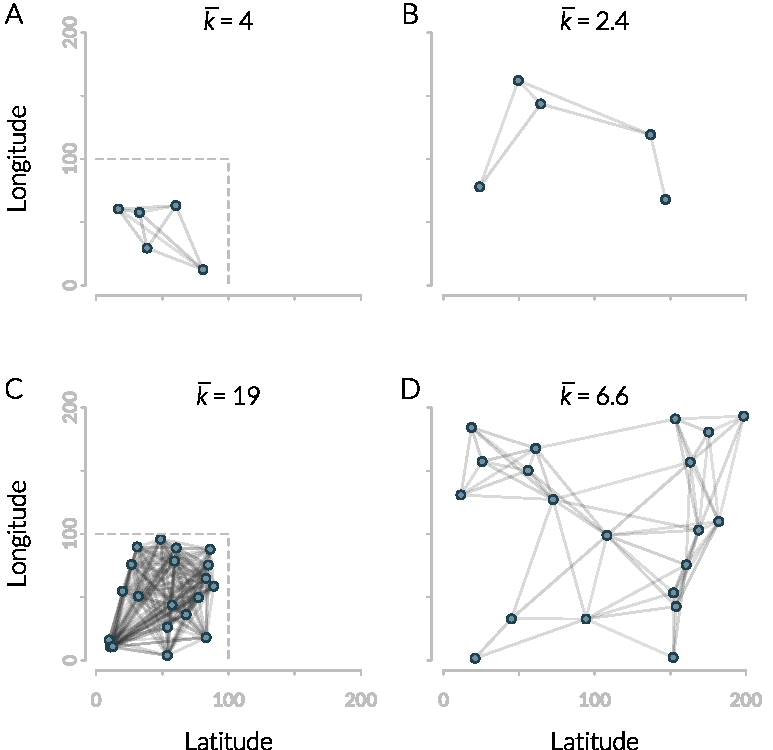
\includegraphics[width=0.9\textwidth]{figure/colonyNetworkPlots-1} 

}

\caption[Relationship between range size and metapopulation network structure]{
The relationship between range size and metapopulation network structure.
Colonies are shown by circles.
Colonies that are close enough for animals to disperse between (i.e.  within \SI{100}{\kilo\meter} of each other) are joined by a line.
Colonies are placed randomly in spaces of various sizes (grey dashed lines).
A and C) the default range size (\SI{10000}{\square\kilo\metre}).
B and D) the largest range size (\SI{40000}{\square\kilo\metre}).
A and B) the smallest number of colonies (five).
C and D) the default number of colonies (20).
The mean number of connections per subpopulation, $\bar{k}$, is shown for each metapopulation.
}\label{fig:colonyNetworkPlots}
\end{figure}


\end{knitrout}











\begin{knitrout}\footnotesize
\definecolor{shadecolor}{rgb}{0.969, 0.969, 0.969}\color{fgcolor}\begin{figure}[t]

{\centering 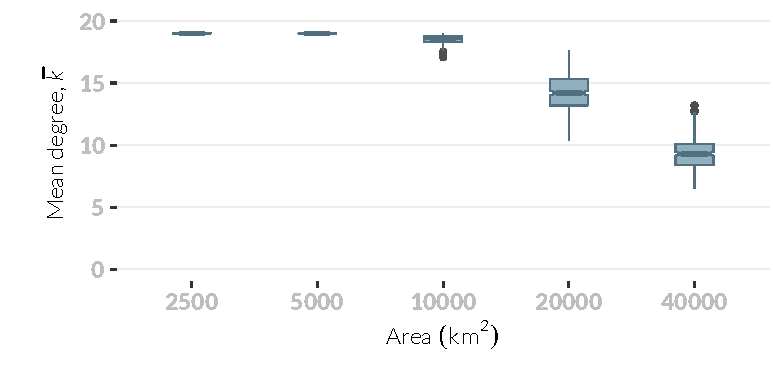
\includegraphics[width=0.8\textwidth]{figure/plotK-1} 

}

\caption[Change in average network degree with increasing range size]{
Change in average metapopulation network degree ($\bar{k}$) with increasing range size. 
Bars show the median, boxes show the interquartile range, vertical lines show the range and grey dots indicate outlier values.
Notches indicate the 95\% confidence interval of the mean.
All simulations had 20 colonies, meaning 19 is the maximum value of $\bar{k}$.
}\label{fig:plotK}
\end{figure}


\end{knitrout}
















\begin{knitrout}\footnotesize
\definecolor{shadecolor}{rgb}{0.969, 0.969, 0.969}\color{fgcolor}\begin{figure}[t]

{\centering 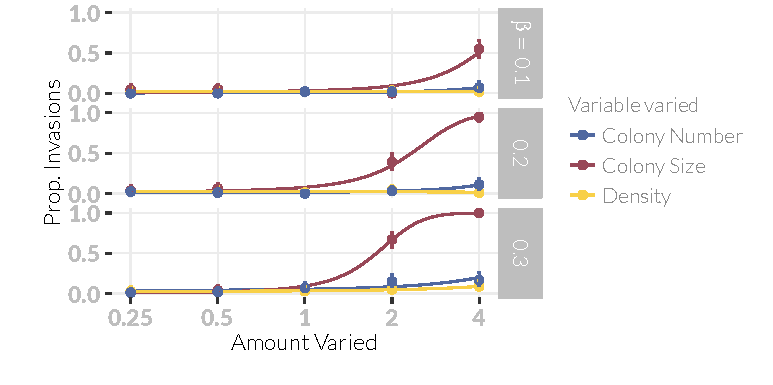
\includegraphics[width=\textwidth]{figure/plotValueChangeMeans-1} 

}

\caption[Comparison of the effect of colony size, number of colonies and host density on probability of invasion.]{
Comparison of the effect of colony size, number of colonies and host density on probability of invasion.
The $x$-axis shows the relative change in the default values of each of these factors ($\times 0.25, 0.5, 1, 2$ and $4$).
Default values are: colony number = 20, colony size = 400 and density = 0.8 animals.\si{\per\square\kilo\metre}.
Red) population size is altered by changing colony number.
Blue) population size is altered by changing colony size.
Yellow) population density is altered by changing range size.
Each point is the mean of 100 simulations and bars are 95\% confidence intervals.
Curves are simple logistic regression fits for each independent variable.
Relationships are shown separately for each transmission value, $\beta$.
}\label{fig:plotValueChangeMeans}
\end{figure}


\end{knitrout}







\begin{knitrout}\footnotesize
\definecolor{shadecolor}{rgb}{0.969, 0.969, 0.969}\color{fgcolor}\begin{figure}[t]

{\centering 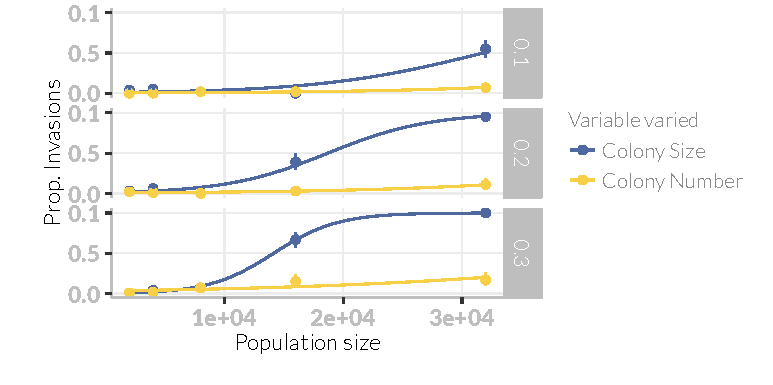
\includegraphics[width=\textwidth]{figure/plotTransMeans-1} 

}

\caption[Comparison of the probability of invasion when host population size is altered by changing colony size or colony number.]{
Comparison of the effect of host population size on probability of invasion when population size is altered by changing colony size or colony number.
Relationships are shown separately for each transmission value, $\beta$.
It can be seen that changes in colony size give a much greater increase in invasion probability than changes in colony number.
Note that this is the same data as Figure~\ref{fig:plotValueChangeMeans} but with the $x$-axis scaled by population size, rather than relative parameter change.
}\label{fig:plotTransMeans}
\end{figure}


\end{knitrout}







%%%%%%%%%%%%%%%%%%%%%%%%%%%%%%%%%%%%%%%%%%%%%%%%%%%%%%%%%%%%%%%%%%%%%%%%%%%%%%%%%%%%%%%%%%%%%%%%%%%%%%%%%%%%%%%%%%%%%%%%%%%%%%%%%%%%%%%%%%%%%%%%%%%%%%%%%%%


\section{Methods}

%%%%%%%%%%%%%%%%%%%%%%%%%%%%%%%%%%%%%%%%%%%%%%%%%%%%%%%%%%%%%%%%%%%%%%%%%%%%%%%%%%%%%%%%%%%%%%%%%%%%%%%%%%%%%%%%%%%%%%%%%%%%%%%%%%%%%%%%%%%%%%%%%%%%%%%%%%%

I used a two-pathogen, metapopulation SIR model to compare the roles of population parameters on pathogen species richness.
The multipathogen SIR model was identical to that in Chapter~\ref{ch:sims1} and an implementation in \emph{R} \cite{R} is available as a package on GitHub \cite{metapopepi}.
Specifically, I let two identical pathogens --- an endemic pathogen and an invading pathogen --- compete and used persistence or not of the Pathogen 2 as my response variable.
I tested whether host population size is more important than host density.
I then tested whether colony size or the number of colonies is the more important component of population size.
I used the same fixed parameters as Chapter~\ref{ch:sims1} (Table~\ref{t:params}) except I used only three values of the transmission rate $\beta$,  0.1, 0.2 and 0.3.
All simulations were run under all three transmission rates.
The code used for running all simulations is available at \url{https://github.com/timcdlucas/PhDThesis/blob/master/Chapter4.Rtex}.

In each simulation the host population was seeded with 20 individuals infected with Pathogen 1 in each colony. 
Pathogen 1 was then allowed to spread and reach equilibrium. 
After \SI{700000} events, five hosts individuals infected with Pathogen 2 were added to one randomly selected colony. 
After another \SI{300000} events the invasion of Pathogen 2 was considered successful if any individuals infected  with Pathogen 2 still remained.

The effect of range size on disease dynamics occured through changes in the metapopulation network.
The metapopulation structure was created for each simulation by randomly placing colonies in a square space (Figure~\ref{fig:colonyNetworkPlots}).
This square space was considered to be the species geographic range, the size of which was varied.
Range size was varied between \SI{2500} and \SI{40000}{\square\kilo\metre}.
This corresponds to square areas with sides of 50 to \SI{200}{\kilo\metre}.
Dispersal was only allowed to occur between two colonies if they are within \SI{100}{\kilo\metre} of each other i.e.\ they were then counted as connected nodes in the metapopulation network.
The number of connections each colony has is called its degree, $k$.
How well connected the metapopulation network is overall is measured by the mean degree, $\bar{k}$.
The random placement of colonies in space did not guarantee that the population network is connected (i.e.\ made up of a single connected component) but as Pathogen 1 was seeded in all colonies, Pathogen 2 could not be seeded into a fully susceptible colony.
This was considered more realistic than repeatedly resampling the colony locations until a connected metapopulation population occurred.
The threshold of \SI{100}{\kilo\metre} was arbitrary but I aimed to maximise the range  of $\bar{k}$ (Figure~\ref{fig:plotK}) while not having many simulations with networks that were not fully connected.
Given this setup, populations with low densities had relatively unconnected metapopulation networks while high density populations had fully connected networks (Figure \ref{fig:plotK}).






\subsection{Population factors}

Three sets of simulations were run (Table~\ref{t:popParams}).
This set of three simulations was used to compare two pairs of population factors: \emph{i}) population size and host density, \emph{ii}) colony size and the number of colonies.
The population parameters that were directly varied were colony size, the number of colonies and range size.
In each case the values these parameters took were their default value multiplied by 0.25, 0.5, 1, 2 and 4.
The default colony size was 400, the default number of colonies was 20 and the default range size was \SI{10000}{{\square\kilo\metre}}.

\subsubsection{Population size and host density}
In the first set of simulations, host density was varied by keeping population constant while varying range size.
Colony size was kept at a constant value of 400 while the number of colonies was fixed at 20 giving a population size of 8000.
The values of range size used were \SI{40000}, \SI{20000}, \SI{10000}, \SI{5000} and \SI{2500}{\square\kilo\metre} which gave density values of 0.2, 0.4, 0.8, 1.6 and 3.2 animals.\si{\per\square\kilo\metre}.

In the second set of simulations, population size was varied by changing colony size while the number of colonies was kept constant.
To keep host density constant, range size was reduced as population size increased.
The values of colony size used were 100, 200, 400, 800 and \SI{600} while range size was set to \SI{40000}, \SI{20000}, \SI{10000}, \SI{5000} and \SI{2500}{\square\kilo\metre}.
This gave population size values of \SI{2000}, \SI{4000}, \SI{8000}, \SI{16000} and \SI{32000} while host density remained at 0.8 hosts{\si{\per\square\kilo\metre}}.

In the third set of simulations, population size was varied by changing the number of colonies while colony size was kept constant.
Again, to keep host density constant, range size was reduced as population size increased.
The numbers of colonies used were 5, 10, 20, 40 and 80 while range size was set to \SI{40000}, \SI{20000}, \SI{10000}, \SI{5000} and \SI{2500}{\square\kilo\metre}.
Again, this gave population size values of \SI{2000}, \SI{4000}, \SI{8000}, \SI{16000} and \SI{32000} while host density remained at 0.8 hosts{\si{\per\square\kilo\metre}}.


\subsubsection{Colony size and the number of colonies}

To compare colony size and the number of colonies, only the second and third set of simulations above were used.
However, colony size and the number of colonies were directly used as independent variables instead of using the derived values for host density or population size.
It can be seen that population density and range size are equivalent in the two sets of simulations.
Therefore, the only difference between these two sets of simulations is the factor used to increase population size: colony size or the number of colonies.




\subsection{Statistical analysis}

I tested two hypotheses.
Firstly I tested the hypothesis that an increase in host population size creates a stronger increase in invasion probability (of the second pathogen) than an equal increase in host density.
Secondly, I tested the hypothesis that an increase in colony size creates a stronger increase in invasion probability than a proportionally equal increase in number of colonies.
To statistically test these hypotheses I combined the results from different simulations and fitted multiple logistic regressions, centering and scaling the independent variables.
Specifically, I fitted the model 
\begin{align}
  \text{Invasion} = b_1 d + b_2 n + b_3 m + c + \epsilon
\end{align}
where $d, n$ and $m$ are density, colony size and number of colonies respectively and $b_i$ are the regression coefficients. 
$c$ is a fitted intercept and $\epsilon$ is a binomially distributed error term.
To test the first hypothesis I compared the size (and 95\% confidence intervals) of $b_1$ to $b_2$ and $b_3$.
To test the second hypothesis I compared $b_2$ to $b_3$.

Logistic regression was also used to test for an affect of transmission rate at the default parameter setting.
Finally, in a small number of simulations both pathogens went extinct.
Logistic regression was used to test whether transmission rate was associated with these events.




%%%%%%%%%%%%%%%%%%%%%%%%%%%%%%%%%%%%%%%%%%%%%%%%%%%%%%%%%%%%%%%%%%%%%%%%%%%%%%%%%%%%%%%%%%%%%%%%%%%%%%%%%%%%%%%%%%%%%%%%%%%%%%%%%%%%%%%%%%%%%%%%%%%%%%%%%%%


\section{Results}

%%%%%%%%%%%%%%%%%%%%%%%%%%%%%%%%%%%%%%%%%%%%%%%%%%%%%%%%%%%%%%%%%%%%%%%%%%%%%%%%%%%%%%%%%%%%%%%%%%%%%%%%%%%%%%%%%%%%%%%%%%%%%%%%%%%%%%%%%%%%%%%%%%%%%%%%%%%



%%%%%%%%%%%%%%%%%%%%%%%%%%%%%
%%%     Results text    %%%%%
%%%%%%%%%%%%%%%%%%%%%%%%%%%%%

At the default parameter settings, the probability of invasion and establishment of the second pathogen, $P(I)$,  was rare (Figure~\ref{fig:plotValueChangeMeans} and Tables~\ref{C-pop}--\ref{C-dens2}).
These proportions significantly increase with transmission rate (GLM: $b$ = 0.18, $p$ = 0.01).

In 37 simulations, both of the pathogens went extinct.
This did not depend on transmission rate (GLM: $b$ = \ensuremath{-0.01}, $p$ = 0.69).
However they were all either in simulations with the smallest colony size (colony size = 100, 29 simulations) or with the fewest colonies (5 colonies, 8 simulations).
Results from these simulations were removed before further analyses.



\subsection{Host density or population size}

To test whether host density or population size had a stronger affect on invasion probability I compared the regression coefficients of the multiple regressions fitted to simulation results (Figure~\ref{fig:plotValueChangeMeans}).
Increasing host population size, either by increasing colony size or number of colonies, increased the probability of invasion (Table~\ref{t:regrCoefs}).
The relationship between colony size and invasion is strong and significant at all transmission rates, while the relationship between colony number and invasion is weaker and more marginally significant.
In contrast, varying host density does not alter invasion probability.
Therefore the simulations support the hypothesis that population size affects invasion more strongly than host density.


\subsection{Colony size or number of groups}

To test whether colony size or the number of colonies is the more important component of population size, I compared the regression coefficients, $b_2$ and $b_3$, of the multiple regressions fitted to simulation results (Figure~\ref{fig:plotTransMeans}).
Increasing either colony size or the number of colonies increased the probability of invasion but this affect was much stronger and more statistically significant for colony size (Table~\ref{t:regrCoefs}).
Therefore the simulations support the hypothesis that colony size is the more important component of population size.




\begin{table}

\caption[Regression results]{
Regression results comparing effects of colony size, colony number and density.
Coefficients are from multiple logistic regressions with invasion as the dependent variable and all independent variables being scaled and centred.
Colony size and colony number were varied while keeping density equal while density was varied by changing range size while keeping population size equal.
$p$ is for the test against the null hypothesis that  $b = 0$.
}
\label{t:regrCoefs}
\centering
\begin{tabular}{@{}rlrrr@{}}
\toprule
$\beta$ & \emph{Variable} & \emph{Estimate} ($b$) & (95\% \emph{CI}) & $p$\\
\midrule
0.1   &    Intercept     & \ensuremath{-3.52} & (\ensuremath{-3.87}, \ensuremath{-3.2}) & $< 10^{-5}$ \\
      &    Colony Size   & 1.07 & (0.75, 1.49) & $< 10^{-5}$ \\
      &    Colony Number & 0.35 & (\ensuremath{-0.02}, 0.79) & 0.08 \\
      &    Density       & 0.01 & (\ensuremath{-0.66}, 0.52) & 0.97 \\[1em]
0.2   &    Intercept     & \ensuremath{-2.84} & (\ensuremath{-3.12}, \ensuremath{-2.58}) & $< 10^{-5}$ \\
      &    Colony Size   & 2.11 & (1.71, 2.6) & $< 10^{-5}$ \\
      &    Colony Number & 0.51 & (0.16, 0.95) & 0.009 \\
      &    Density       & \ensuremath{-0.31} & (\ensuremath{-0.96}, 0.19) & 0.29 \\[1em]
0.3   &    Intercept     & \ensuremath{-2.11} & (\ensuremath{-2.34}, \ensuremath{-1.9}) & $< 10^{-5}$ \\
      &    Colony Size   & 2.74 & (2.35, 3.16) & $< 10^{-5}$ \\
      &    Colony Number & 0.25 & (0.04, 0.48) & 0.02 \\
      &    Density       & 0.27 & (\ensuremath{-0.06}, 0.57) & 0.09 \\

\bottomrule

\end{tabular}
\end{table}



%%%%%%%%%%%%%%%%%%%%%%%%%%%%%%%%%%%%%%%%%%%%%%%%%%%%%%%%%%%%%%%%%%%%%%%%%%%%%%%%%%%%%%%%%%%%%%%%%%%%%%%%%%%%%%%%%%%%%%%%%%%%%%%%%%%%%%%%%%%%%%%%%%%%%%%%%%%


\section{Discussion}

%%%%%%%%%%%%%%%%%%%%%%%%%%%%%%%%%%%%%%%%%%%%%%%%%%%%%%%%%%%%%%%%%%%%%%%%%%%%%%%%%%%%%%%%%%%%%%%%%%%%%%%%%%%%%%%%%%%%%%%%%%%%%%%%%%%%%%%%%%%%%%%%%%%%%%%%%%%

\tmpsection{Restate results}

Overall, my results suggest that population size promotes pathogen richness significantly more than host density in the context of metapopulations or group living.
Furthermore, the component of population size that is important is colony size.

These results lead to a number of other conclusions.
All else being equal, increasing range size (with density remaining constant) will not strongly increase pathogen richness unless the increased range size promotes larger groups.
Furthermore, social species that live in large groups are likely to harbour more pathogen species, even if 
the larger groups require more space and therefore dispersal between groups is reduced.

\tmpsection{Why are these results like that? What do they mean?}

The results suggest that, for related, strongly competing strains, the factor that most strongly allows new pathogens to invade is the number of susceptible individuals in the local group.
As long as there are enough susceptible individuals that the new pathogen species persists through the stochastic, early stages of the epidemic, the new pathogen will persist.
As dispersal is a very slow process compared to infection, the global pool of susceptibles is not important. 
This is probably why increasing the number of colonies did not increase pathogen invasion rate as quickly as the size of a colony did.
Similarly, the global host density of the species had little effect on pathogen invasion rate.
In these simulations, increasing density without increasing population size was only achieved by reducing range size; this simply increased the number of connections between colonies in the metapopulation network.
This, in turn, increased the pool of susceptibles that were within one dispersal of the invading pathogen.
However, again, this effect was very weak compared to the strong changes in local disease dynamics caused by increasing colony size.



\subsection{Global change}

It is clear that many species are suffering strong population changes due to global change \cite{thomas2004extinction}.
However these changes might affect range size \cite{thomas2004extinction}, population size \cite{craigie2010large}, population connectivity \cite{wasserman2013population, rivera2015habitat, fonturbel2014forest} or group size \cite{lehmann2010apes, zunino2007habitat, manor2003impact, atwood2006influence} to different extents.
My results suggest that pathogen communities will respond differently depending on which factors are affected most affected by global change.
In short, species suffering reductions in groups size \cite{lehmann2010apes, zunino2007habitat, manor2003impact, atwood2006influence} are predicted to experience decreases in pathogen richness in the long term and there is some evidence that this process is occurring \cite{altizer2007threatened, turmelle2009correlates}.
Species that are experiencing increases in group size \cite{lehmann2010apes} would be expected to gain new pathogen species.
In contrast, species suffering range contractions \cite{thomas2004extinction} and decreases in population size \cite{craigie2010large} are expected to experience smaller changes in pathogen richness.
However, it should be noted that these conclusions apply only to the specific mechanism studied here; the invasion of newly evolved pathogens.

\subsection{Comparative studies}

Many comparative studies measure some aspect of a species population size or structure, yet it is rarely discussed how these relate.
Instead most studies use the data that are available, without considering \emph{a priori} how the explanatory variables are causally related (though statistical correlations between independent variables is usually considered and dealt with using PCA or by removing colinear variables).
Host density is often measured \cite{morand1998density, lindenfors2007parasite, nunn2003comparative, arneberg2002host} yet density is directly associated with population size.
This study suggests that it is in fact population size that is important (in the context of social species as studied here).
This suggests that the density measures in these comparative studies are in fact proxies for population size rather than the true causal factor.
Similarly, this study suggests that host range size does not promote pathogen richness by the mechanism studied here, yet a number of studies have found evidence of this relationship \cite{kamiya2014determines, nunn2003comparative}.
This suggests that either the relationship found in comparative studies is in fact due to a correlation with another factor, or that mechanisms other than probability of invasion of new pathogens are important.
Range size has been suggested to affect pathogen richness by a number of mechanisms such as increasing the number of sympatric species and these other mechanisms should be specifically tested \cite{luis2013comparison}.

The studies that have specifically tested the effect of group size have in fact found both positive \cite{vitone2004body} and negative associations \cite{gay2014parasite} or no relationship \cite{ezenwa2006host}.
Meta-analyses suggest that the relationship between social group size and pathogen richness is weak \cite{rifkin2012animals}.
However, I have found that group size is the most important population factor.
This suggests that the mechanism studied here --- invasion of recently evolved pathogens --- may not the major mechanism by which pathogen richness is created in wild populations.



\subsection{Assumptions and limitation}

Being based on the same model as used earlier, the work presented here relies on many of the same assumptions (see Section~\ref{s:sims1Disc}).
Furthermore, as a comparison is being made between the effects of range size and population size, the exact specifications of how the metapopulation is affected by range size is important.
I have conducted this study at one rate of dispersal, 0.01 dispersals per individual per year.
In practice this relates to only 17\% of individuals dispersing in their lifetime.
This low rate of dispersal is expected to exaggerate the effect of range size; at high rates of dispersal the population is essentially well-mixed, despite the metapopulation.

Furthermore, there is evidence that as groups get bigger, the within-group structure increases \cite{nunn2015infectious}.
This has not been modelled here; instead the subpopulations are assumed to be fully mixed regardless of size.
Also, I have assumed that dispersal only occurs between colonies a certain distance apart.
Based on \emph{a priori} considerations such as the time and energy required to disperse long distances this is a reasonable assumption.
The exact threshold was chosen to attempt to maximise the range of $\bar{k}$ studied (Figure~\ref{fig:plotK}).
However, a similar assumption could be made in other ways.
Instead of a threshold distance, individuals could be expected to disperse in a random direction and stop at the first colony they encounter; this could create some long distance links in the network and increase network connectivity, potentially reducing the effects of range size.
Alternatively, the metapopulation could have been modelled as a weighted network with dispersal occurring at a higher rate to nearby colonies.
Depending on the parameterisation of this distance-dispersal relationship this could serve to increase the affect of range size --- by exaggerating dispersal to very nearby colonies --- or decrease the affect of range size by allowing rare, but significant, global dispersal creating a small-world network structure.
Ultimately, the modelling choices could increase or decrease the affects of range size relative to colony size and the number of colonies but I have aimed to make the effect of range size as strong as possible.




\tmpsection{Further correlations between factors}

I have used the simple relationships between demographic factors --- $d = N / a$ for example --- to illustrate that these are tightly linked.
In order to isolate the effects of these factors I have assumed these simple relationships hold; to examine density without altering population size I have fixed population size and manipulated range size.
However, in reality, these are likely to covary both within species across time and also between species.
Therefore, while these quantities are certainly linked, they cannot be assumed to have simple linear relationships and should not be used as proxies of each other without further examination.
For example, rates and distances of dispersal --- which affect the influence of space --- may be related to local density \cite{marjamaki2013local}.
Similarly it is unlikely that a species whose range size decreases will not experience a decrease in total population size as well; the range contraction is likely to occur over generations rather than a simple squeezing of the existing individuals into a smaller area.




\subsection{Conclusions}

Overall I have shown that while a number of demographic factors are intrinsically linked, they have different effects on the rate at which new pathogens will invade.
I found that population size, not density, has the stronger impact on the ability of a pathogen to invade.
Furthermore, species with large groups are likely to harbour more pathogens than species with many, smaller groups.
Due to the correlations between these factors, they are particularly hard to study within a comparative framework; this highlights the utility of mechanistic models.








%%%%%%%%%%%%%%%%%%%%%%%%%%%%%%%%%%%%%%%%%%%%%%%%%%%%%%%%%%%%%%%%%%%%%%%%%%%%%%%%%%%%%%%%%%%%%%%%%%%%%%%%%%%%%%%%%%%%%%%%%%%%%%%%%%%%%%%%%%%%%%%%%%%%%%%%%%%


%\section{Appendix}

%%%%%%%%%%%%%%%%%%%%%%%%%%%%%%%%%%%%%%%%%%%%%%%%%%%%%%%%%%%%%%%%%%%%%%%%%%%%%%%%%%%%%%%%%%%%%%%%%%%%%%%%%%%%%%%%%%%%%%%%%%%%%%%%%%%%%%%%%%%%%%%%%%%%%%%%%%%

